%!TEX root = ../CombinatoricsNotes.tex

\section{The Littlewood-Offord problem}
\lect{1}{18}
% \marginnote{Lecture 4: Monday, January 18, 2014.}

\begin{problem}[\cite{LO1943}]
Given $(z_1,\dotsc,z_n)$ complex numbers, with $|z_i| \geq 1$. Consider the $2^n$ possible sums formed by the $z_i$'s. How many sums can have pairwise distances less than 1 from each other? If $z_1 = z_2 = \dotsc =z_n=1$, then we get ${n \choose \floor{n/2}}$ equal sums.

Given $(z_1,\dotsc,z_n)$, and subset of indicies $A\subset [n]$, let $Z_A = \sum_{i\in A} z_i$, where we define  $Z_\emptyset = 0$ and $Z_{\{i\}} = z_i$. We say $\F \subset \P([n])$ is \defn{Littlewood-Offord}[Littlewood-Offord!sets of numbers] (LO) with respect to $(z_1,\dotsc,z_n)$ if $|Z_A- Z_B| < 1$ for all $A,B \in \F$. In this notation, we are looking for the largest collection $\F$ such that $\F$ is LO with respect to $(z_1,\dotsc,z_n)$.
\end{problem}

\begin{conjecture*}
If $(z_1,\dotsc,z_n) \in \C^n$ with $|z_i|\geq 1$, and $\F$ is LO with respect to $(z_1,\dotsc,z_n)$, then $|\F| \leq {n \choose \floor{n/2}}$.
\end{conjecture*}
\begin{remark}
Littlewood and Offord were not combinatorialists; instead they were interested in studying the roots of random polynomials.
\end{remark}

\begin{theorem}[\cite{erdos1945}]
If $x_1,\dotsc,x_n$ are real, $|x_i| \geq 1$ for every $i$, and $\F$ is LO with respect to $(x_1,\dotsc,x_n)$, then $|\F| \leq { n\choose \floor{n/2}}$.
\end{theorem}
\begin{proof}	
We'll change notation to $X_A$ instead of $Z_A$ for this real case. If $x_1,\dotsc,x_n \geq 1$, then $\F$ is Sperner. Suppose $A\subsetneq B$; then
\[
|X_A - X_B| = X_B - X_A = X_{B\setminus A} \geq |B-A| \geq 1. \qquad \checkmark
\]

The general problem for reals can be reduced to this case of $x_i>0$ as follows.
Suppose that $\F$ is LO with respect to $(x_1,\dotsc,x_n)$. Then we will construct a family $\F'$ which is LO with respect to \\$(x_1,\dotsc, x_{i-1},-x_i, x_{i+1}, \dotsc, x_n)$ with $|\F'| = |\F|$. This will suffice to prove the theorem.

Let $\F' = \{ A \symd \{i\}: A\in \F\}$\sidenote[][]{We remove $i$ if it's there, and add it otherwise.}. Clearly $|\F'| = |\F|$. We've reduced all sums by $x_i$, as shown by the following. If $i \in A$, then $X'_{A \symd \{i\}} = \left(\sum_{j\in A} x_j \right)-x_i$. if $i \not \in B$, then $X'_{B \symd \{i\}} = \left( \sum_{j\in B} x_j \right) - x_i$.
Hence, all sums are still within $1$ of each other, completing the proof.
\end{proof}



\begin{definition}
A chain $A_1 \subset A_2 \subset \dotsc \subset A_k$ in $\P([n])$ is \defn{symmetric}[symmetric!chain] if $|A_{i+1}| = |A_i| +1$ for $i=1,\dotsc,k-1$. Additionally, we require $|A_1| + |A_k| = n$. 
\end{definition}
Note that in particular, a symmetric chain  intersects $[n]^{(\floor{n/2})}$. An example of symmetric chains is shown in \cref{fig:sym_chains}.
\begin{figure}[ht]
\begin{center}
 \begin{tikzcd}[column sep=tiny]
{[3]}^{(3)}  & &\{1,2,3\}\arrow[green,dash]{ld} \\
{[3]}^{(2)} &\{1,2\} \arrow[dash,green]{d}& \{1,3\}  \arrow[dash,blue]{rd} & \arrow[dash,red]{ld} \{2,3\} \\
\mathbf{[3]^{(1)}} & \mathbf{\{1\}} \arrow[dash,green]{rd} & \mathbf{\{2\}}&\mathbf{\{3\}}\\
{[3]}^{(0)} & & \emptyset
\end{tikzcd}
 \begin{tikzcd}[column sep=tiny]
&\{1,2,3\}\arrow[red,dash]{rd} \\
\{1,2\} \arrow[dash,green]{d}& \{1,3\}  \arrow[dash,blue]{rd} & \arrow[dash,red]{ld} \{2,3\} \\
 \mathbf{\{1\}} \arrow[dash,green]{rd} & \mathbf{\{2\}}&\mathbf{\{3\}}\\
 & \emptyset
\end{tikzcd}
\end{center}
\caption{\textit{Left:} We draw our favorite $\P([n])$, partioned into symmetric chains, which thus each intersect $[n]^{(\floor{n/2})}$. \textit{Right:} A partition of $\P([n])$ into chains which intersect $[n]^{(\floor{n/2})}$, which we could obtain from the proof of \cref{thm:sperner}. But these chains are not symmetric.} \label{fig:sym_chains} 
\end{figure}

Our previous method, when proving Sperner's theorem, didn't actually guarantee symmetric chains; see \cref{fig:sym_chains}. We will do this now, which provides a new proof of Sperner's theorem.

\pagebreak
\begin{theorem} \label{thm:sym_part}
$\P([n])$ can be partitioned into symmetric chains.
\end{theorem}
\begin{proof}[Proof by induction on $n$.]
 The base case $n=1$ is immediate.
Induction step: Let $C_1,C_2,\dotsc,C_L$ be symmetric chains forming a partition of $\P{[n-1]}$. Consider $C_i = (A_1,A_2,\dotsc,A_k)$. Form 
\begin{align*}	
 C_i' &= (A_1,A_2,\dotsc,A_k,A_k\cup \{n\})\\
 C_i'' &= (A_1 \cup \{n\}, A_2 \cup \{n\}, \dotsc, A_{k-1} \cup \{n\}).
 \end{align*} 
 % \improvement{Add picture of $n=3$ of $C_i'$ and $C_i''$.}
 \begin{figure}
 \begin{center}
 \begin{tikzcd}[column sep=tiny]
% {[n]}^{(3)}  & &\{1,2,3\}\arrow[green,dash]{ld} \\
\phantom{{[n]}^{(3)}}& & \\
{[2]}^{(2)} &\{1,2\} \arrow[dash,OliveGreen]{d}&  \\
\mathbf{[2]^{(1)}} & \mathbf{\{1\}} \arrow[dash,OliveGreen]{rd} & \mathbf{\{2\}}&\\
{[2]}^{(0)} & & \emptyset
\end{tikzcd}\hfill
\begin{tikzcd}[column sep=tiny]
{[3]}^{(3)}  & &\{1,2,3\}\arrow[DarkGreen,dash]{ld} \\
{[3]}^{(2)} &\{1,2\} \arrow[dash,DarkGreen]{d}& \{1,3\}  \arrow[dash,LightGreen]{rd} & \arrow[dash,red]{ld} \{2,3\} \\
\mathbf{[3]^{(1)}} & \mathbf{\{1\}} \arrow[dash,DarkGreen]{rd} & \mathbf{\{2\}}&\mathbf{\{3\}}\\
{[3]}^{(0)} & & \emptyset
\end{tikzcd}
\end{center}
\caption{An illustration of the induction step, from $n=2$ on the left to $n=3$ on the right. On the left,  two chains: $C_1 = (\emptyset, \{1\}, \{1,2\})$ in green, and $C_2 = (\{2\})$.
We create $C_1' = (\emptyset, \{1\},\{1,2\},\{1,2,3\})$ in dark green, and $C_1'' = (\{3\}, \{1,3\})$ in light green. We also create $C_2' = (\{2\},\{2,3\})$ in red, and $C_2'' = ()$, an empty chain.%
}%
 \end{figure}
We can easily see that given that $C_i$ was a symmetric chain on $\P([n-1])$, we have $C_i'$ and $C_i''$ are both symmetric chains on $\P([n])$. Moreover, 
\[
\{C_1', \dotsc, C_L'\}\cup \{C_1'', \dotsc, C_L''\}
\]
form a partition of $\P([n])$, as follows:  For any set $A\in \P([n])$, if $n\not \in A$, then $A\in C_i$ for some $i$, and hence $A\in C_i'$. If $n\in A$, then $A\setminus \{n\} \in C_i = (A_1,A_2,\dotsc,A_k)$ for some $i$, so $A = A_j$ for some $j$. If $j=k$, then $A\in C_i'$, otherwise $A\in C_i''$. In any case, if $A\in \P([n])$, $A$ is in one of these chains. Finally, $A$ cannot be in two chains, otherwise we have that $\{C_i\}$ was not a partition of $\P([n-1])$.
\end{proof}

Any partition of $\P([n])$ symmetric chains has ${n\choose \floor{n/2}}$ sets, because each chain must intersect with one point in $[n]^{(\floor{n/2})}$.
In the proof, we took a partition into ${n-1 \choose \floor{(n-1)/2}}$ chains, and seem to have created $2 {n-1 \choose \floor{(n-1)/2}} \neq {n\choose \floor{n/2}}$ chains. The catch is that $C_i''$ is an empty chain if $k=1$.


\newthought{Let us count} the sizes of symmetric chains. Suppose $C_1,\dotsc,C_L$ is a partition of $\P([n])$ into symmetric chains, where $L = {n\choose \floor{n/2}}$. How many chains are there of length $r=n+1$ in the partition? Exactly one, the chain which contains the empty set and must therefore contain the set of $n$ elements.

What about $r=n$? Zero.

What about $r= n-1$? $n-1$ chains, because it must start the collection of 1 element sets and go to the collection of $n-1$ element sets. There are $n$ 1-element sets, but one is already in the maximal chain, so we are left with $n-1$.

What about $r= (n+1)-2i$? These are the symmetric chains which start at the $i$th level $[n]^{(i)}$ and go to the $n-i$th level $[n]^{(n-i)}$. The result is ${n\choose i} - {n\choose i-1}$. That is because there are ${n\choose i}$ elements in $[n]^{(i)}$, but ${n\choose i-1}$ of them are part of longer chains, the number of which is the number of elements in the level $[n]^{(i-1)}$.

Let us formulate analogues of these ideas to solve the Littleword-Offord problem in $\R^d$.
\begin{theorem}[\cite{KLEITMAN1970}] \label{thm:kleit70}
Let $(x_1,\dotsc,x_n)$ be vectors in $\R^d$, with $\|x_i\| \geq 1$. As before, define for $A\subset [n]$, $X_A = \sum_{i\in A} x_i$, and say that $\F\subset \P([n])$ is \defn{LO}[Littlewood-Offord!sets of vectors] with respect to $(x_1,\dotsc,x_n)$ if for each $A,B\in \F$, we have $\|X_A - X_B\| < 1$.
Let $\F$ be LO with respect to $(x_1,\dotsc,x_n)$. Then $|\F| \leq { n\choose \floor{n/2}}$.
\end{theorem}
\begin{proof}	
We will say $\Cset\subset \P([n])$ is \defn{sparse}[sparse!set of indicies of vectors] (with respect to $(x_1,\dotsc,x_n)$) if $\|X_A-X_B\| > 1$ for all $A,B\in \Cset$ with $A\neq B$.x
It is enough to show that $\P([n])$ can be partitioned into ${n\choose \floor{n/2}}$ sparse sets\sidenote{A LO family may only contain one element of each sparse set.}. 

We say that a partition $C_1,\dotsc,C_L$ of $\P([n])$ is \defn{symmetric}[symmetric!partition] if it contains exactly ${n\choose i} - {n\choose i-1}$ ``chains'' of order $(n+1)-2i$ for $i=0,1,\dotsc,\floor{n/2}$, and no chains with sizes not congruent to $n+1 \mod 2$. \marginnote{Here, ``chain'' simply means a set $C_i$ for some $i\in [L]$.}  In particular, $L= {n\choose \floor{n/2}}$.

We will show that $\P[n]$ has a symmetric partition into sparse sets. Then we will have found $L = {n\choose \floor{n/2}}$ sparse sets, completing the proof.
Let's proceed by induction on $n$. For $n=1$, we have $X_\emptyset = 0$, and $X_{\{1\}} = x_1$. Then $\{\emptyset, \{1\}\}$ is sparse if $\|X_\emptyset - X_{\{1\}}\| > 1$, which holds because $\|x_1\| > 1$.
Induction step: Let $C_1,C_2,\dotsc, C_L$ be a symmetric partition of $\P([n-1])$ into sets sparse with respect to $(x_1,\dotsc,x_{n-1})$. 

Let $C_i = \{A_1,\dotsc,A_k\}$. We'd like to form sparse sets
\begin{align*}	
C_i' &= \{A_1,A_2,\dotsc,A_k,A_k \cup \{n\}\}\\
C_i'' &= \{A_1\cup \{n\}, A_2\cup\{n\},\dotsc,A_{k-1}\cup \{n\}\}.
\end{align*}
Our sets $A_1,\dotsc,A_k$ do not have an ordering this time, and we may choose any set to be $A_k$. We will have to use this freedom; consider translating the sums in some chain $C_i = (A_1,\dotsc,A_k)$ by adding the vector $x_n$. We want $C_i'$ to be sparse, but then we need $X_{A_k\cup\{n\}}$ far from each $X_{A_j}$, which does not always need to happen, as illustrated in \cref{fig:LO_proof_prob}.
\begin{marginfigure}[-3cm]
%!TEX root = ../Combinatorics.tex

\newcommand{\makearrow}[2]{
    \begin{scope}
    \coordinate (A) at (#1);
    \coordinate (B) at ([xshift=+120pt,yshift=+60pt]A);
    \draw (A) edge[->] (B);
\end{scope}
}

\newdimen\XCoord
\newdimen\YCoord

\newcommand*{\ExtractCoordinate}[1]{\path (#1); \pgfgetlastxy{\XCoord}{\YCoord};}%
\newcommand*{\LabelCurrentCoordinate}[2]{\fill [#1] ($(\XCoord,\YCoord)$) circle (2pt) node [right] {#2}}%

\pgfmathsetseed{3}

\begin{center}
\begin{tikzpicture}[scale=.25]
\def\scale{.1};
\def\x{2};
\def\y{5};

\coordinate (A) at (\x,\y);
\coordinate (B) at ([xshift=+120pt,yshift=+60pt]A);
\draw (A) edge[->,Red] node[auto=right, pos=-0.1]{{\tiny $X_{A_k}$}} node[ auto=right, near end]{{\tiny $X_{A_k\cup\{n\}}$}} (B);

\coordinate (C) at ($ (A) + (4,4) $);
\coordinate (D) at ([xshift=+120pt,yshift=+60pt]C);

\draw (C) edge[->,Blue] node[auto, near start]{{\tiny $X_{A_1}$}} node[ auto=right, near end]{{\tiny $X_{A_1\cup\{n\}}$}} (D);



\dimline[label style={above=0.5ex},extension start length=.24,extension end length=.24]{($ (A) + .24*(-4,4) $)}{($ (C) + .24*(-4,4) $)}{{\tiny $>1$}};

\coordinate (new) at ($ (C) - (B) $);

\ExtractCoordinate{$(new)$};

\coordinate (newer) at ($(\YCoord,-\XCoord)$);
%(\YCord, -\XCord)


\dimline[label style={ above=.2ex,right, rotate=90},extension start length=-.6,extension end length=-.6]{($ (B) + 3*(newer) $)}{($ (C) + 3*(newer) $)}{{\tiny $<1$}};


% \end{scope}

 % \begin{scope}[scale=\scale]
    % \coordinate (C) at $(\x + 10, \y)$;
    % \coordinate (D) at ([xshift=+120pt,yshift=+60pt]C);
    % \draw (C) edge[->] (D);
% \end{scope}

  \foreach \x in {1,2,...,5}{
    \makearrow{rand*5+4,rand*5-2.5}{\scale};}

\makearrow{3,12}{\scale};
\end{tikzpicture}
\end{center}

% 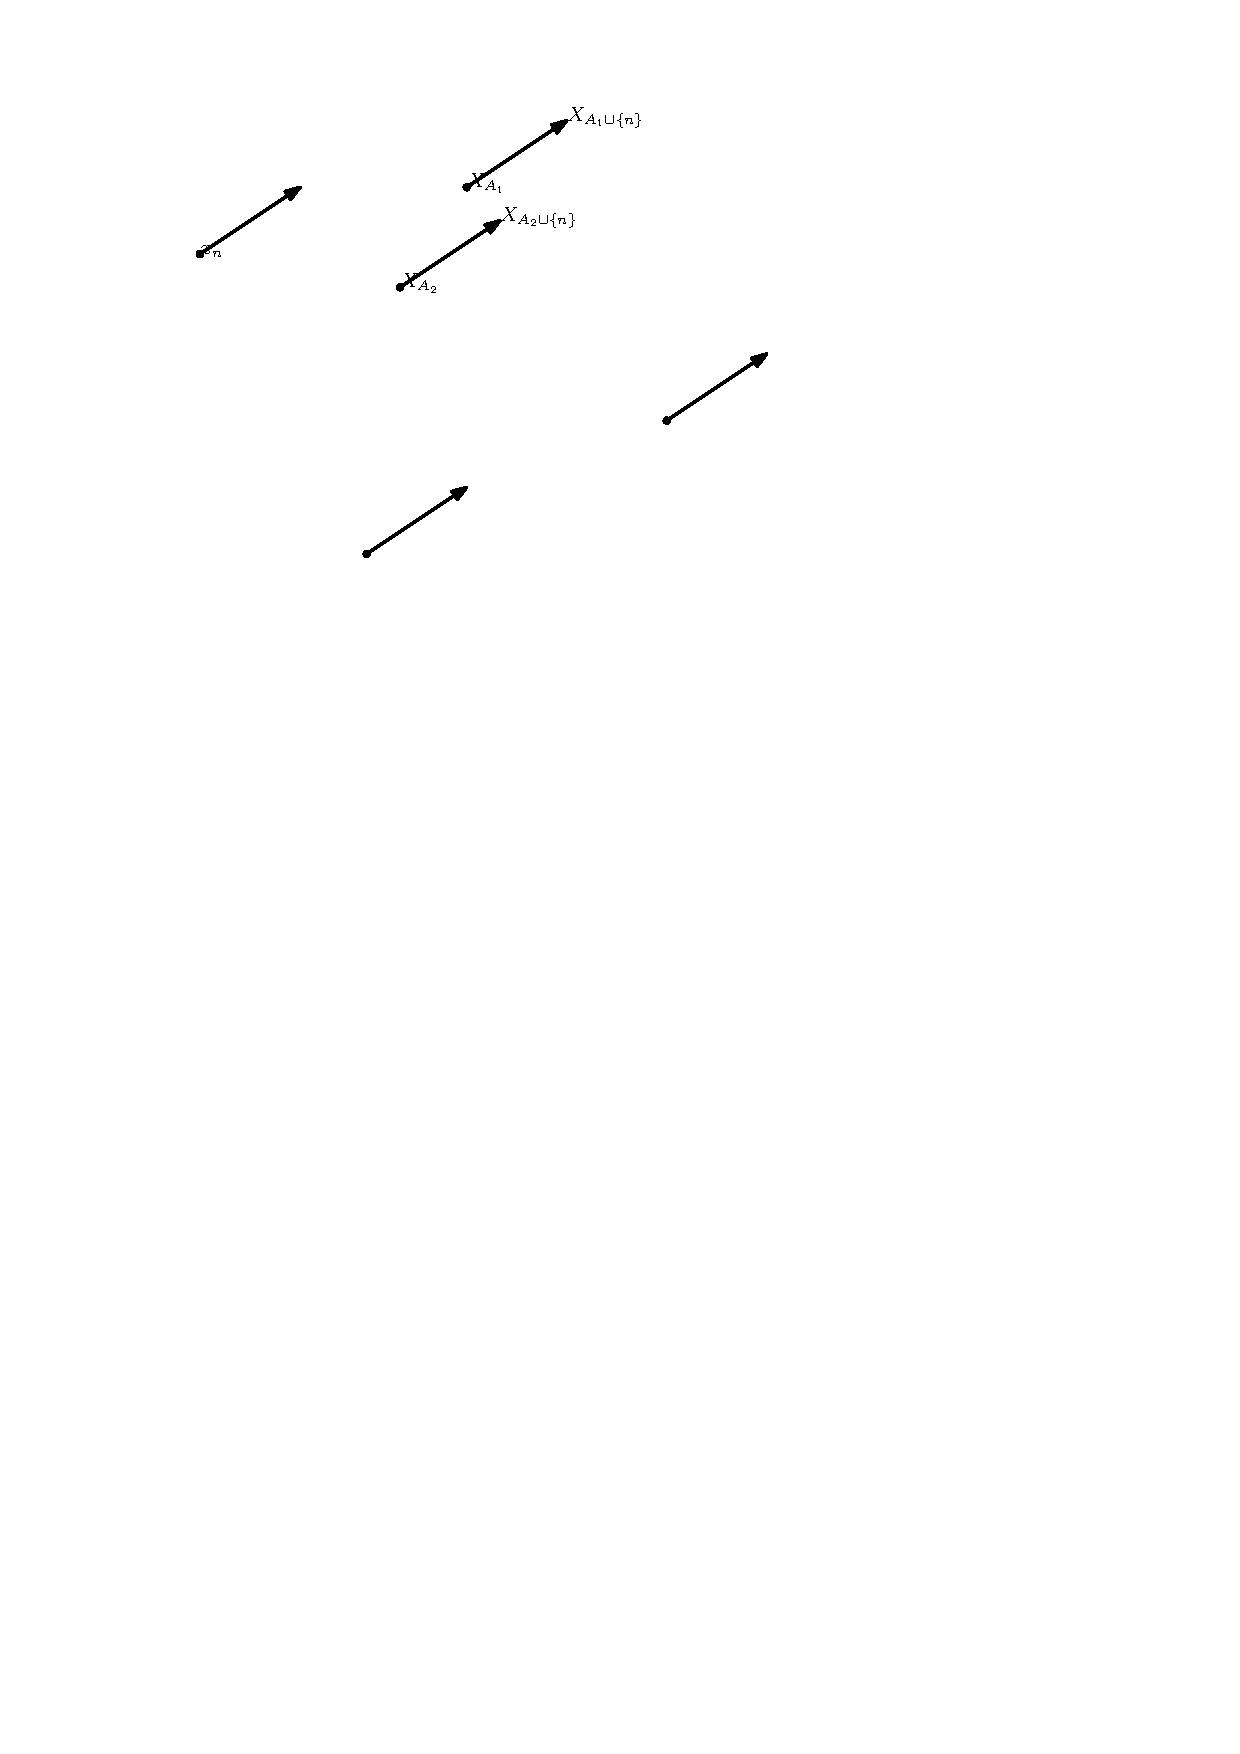
\includegraphics[scale=.5]{graphics/LOproof.pdf}
\caption{With the choice of $A_k$ shown here, we have that $X_{A_k \cup \{n\}} = X_A + x_n$ (in red) is near to $X_{A_1}$ (in blue), so $C_i'$ is not a sparse chain, even though $C_i$ is a sparse chain (all the start points of the arrows are far from each other).} \label{fig:LO_proof_prob}

\end{marginfigure}
% \improvement{Draw better figure, show that the distance is less than 1 in that one spot.}
Assume WLOG that $x_n = (\alpha,0,0,\dotsc,0)$ only has non-zero first coordinate with $\alpha>0$. Let $p(v)$ denote the first coordinate of $v$. Then $p$ is a linear function, and $p(v) \leq \|v\|$ for each $v$. 

Let $A_k$ in the construction above be chosen so that $p(X_{A_k})\geq p(X_{A_j})$ for each $j$\sidenote{So we are choosing $A_k$ to be the furthest in the direction $x_n$. Then if we add $x_n$, we are only moving it further away from the others, so the conflict in \cref{fig:LO_proof_prob} doesn't occur.}. Then to show that $C_i'$ is sparse, it suffices to see that
\begin{align*}	
\|X_{A_k \cup\{n\}} - X_{A_j}\| &\geq p( X_{A_k \cup \{n\}} - X_{A_j})\\
&= p(x_{A_k}) + p(x_n) - p(X_{A_j})\geq p(x_n)\geq 1.
\end{align*}
Hence, we follow the same proceedure as in \cref{thm:sym_part} to conclude that indeed we did produce a symmetric partition.
% \improvement{Add more words to that proof, 2.2.}
\end{proof}


\lect{1}{20}
% \marginnote{Lecture 5: Wednesday, January 20, 2016.}
\newthought{Let us now consider} $\Z_p:=\Z/p\Z$, the integers modulo a prime $p$. Let $x_1,\dotsc,x_n\in \Z_p\setminus\{0\}$. We will say $\Cset \subset \P([n])$ is \defn{sparse}[sparse!set of indicies of integers modulo $p$] with respect to $x_1,\dotsc,x_n$ if $X_A\neq X_B$ for all $A,B\in \C$ with $A\neq B$.
Let us define
\[
\Sigma(z):= | \{A\subset \P([n]): X_A=z\}|.
\]
We are interested in $\max \Sigma(z)$. First, if each $x_1=\dotsb=x_n=1$, then we see that may achieve ${n \choose \floor{n/2}}$.
On the other hand, since there are $2^n$ possible sums and only $p$ values, we have by the pigeonhole principle that $\max \Sigma(z) \geq 2^n/p$. To determine $\max \Sigma(z)$ we will use a partition into sparse sets, just as in the proof of \cref{thm:kleit70}.
\begin{theorem}
Given $x_1,\dotsc,x_n\in \Z_p\setminus\{0\}$ for prime $p$, with $n\leq p-1$, then there exists a symmetric partition of $\P([n])$ into sparse sets with respect to $x_1,\dotsc,x_n$.
\end{theorem}
\begin{proof}	
By induction on $n$. If $\Cset = \{A_1,\dotsc, A_k\}$ is sparse with respect to $x_1,\dotsc,x_{n-1}$, we want to show that
\begin{align*}	
\Cset' &= \{A_1,\dotsc, A_k, A_{\ell} \cup \{n\}\},\\
\Cset'' &= \{A_1\cup \{n\}, A_2\cup\{n\}, \dotsc, A_k \cup \{n\}\}\setminus \{A_\ell \cup \{n\}\}
\end{align*}
 are sparse for some $\ell$. Set $Y_i = X_{A_i}$ and consider the sums $Y_1,\dotsc,Y_k$. We wish to find $1\leq \ell\leq k$ such that $Y_\ell+x_n \not\in \{Y_1,\dotsc,Y_k\}$. Note that $k\leq (n-1)+1 \leq p-1$. Suppose there is no such $\ell$. Then wlog, $Y_1 + x_n = Y_2$, $Y_2 + x_n = Y_3$, \ldots, $Y_j + x_n = Y_1$ for some $j$.

 Then $Y_1 + j x_n = Y_1$, so $jx_n=0$. Then $j=0$ or $x_n = 0$, which is a contradiction, since $j\leq k\leq p-1$.

 In other words, if we have a set $A\subset \Gamma$ for some group $\Gamma$, and for some element $x\in \Gamma$ we have $x+A \subset A$. Then $A$ is a union of cosets of a cyclic subgroup of $\Gamma$ generated by $\{x\}$.
\end{proof}

\begin{corollary} Let $x_1,\dotsc,x_n\in \Z_p\setminus\{0\}$ with $n\leq p-1$.
~\begin{enumerate}
	\item  Then $\Sigma(z) \leq {n \choose \floor{n/2}}$.
	\item (Cauchy-Davenport). Let $S(x_1,\dotsc,x_n) = \{ X_A: A\in \P([n])\}$. Then $|S(x_1,\dotsc,x_n)| \geq \min\{ p,n+1\}$.
\end{enumerate}

\end{corollary}
\begin{proof}	
~ \begin{enumerate}
	\item  A symmetric partition has exactly ${n\choose \floor{n/2}}$ parts, and within each part there is at most one set with corresponding sum $z$.
	\item If $n\leq p-1$, then we have a symmetric partition, which contains a sparse set of size $n+1$. If $n\geq p$, then $S(x_1,\dotsc,x_n) = \Z_p$. This is because we can just use any $p-1$ elements to get all the elements by sums.\qedhere
\end{enumerate}
\end{proof}